\section{Finite populations: count accuracy and mass-distribution discrepancy}
\label{sec:finite}

The critical continuum equation conserves particle count while its mass law
escapes every fixed size window. A finite system has an additional constraint:
no particle can exceed the system's entire mass. This ceiling separates the
finite mass distribution from a growing-time continuum approximation, even
while the count prediction remains accurate. The comparison below starts from
exactly the same empirical measure; it contains no initial sampling error.

The result should be read against the convergence literature for
Marcus--Lushnikov particle systems. Hydrodynamic limits on a fixed time
horizon are classical: \citet{Norris1999} proves such a limit for the
stochastic coalescent, and \citet{Aldous1999} surveys the mean-field theory.
For the additive kernel the stochastic time scale is logarithmic in the
population size: \citet{AldousPitman1998} obtain the standard additive
coalescent by starting the $n$-cluster additive coalescent at time
$-\tfrac12\log n$, so that clusters carrying a positive fraction of the total
mass appear at times of order $\tfrac12\log n$ after the start from $n$ unit
clusters (with $b=1$ their pair rates coincide with those of the process
below without fragmentation). Discrete deterministic mean-field models are
surveyed by \citet{Wattis2006}. \Cref{thm:finite-discrepancy} is a
growing-time statement of a different kind. It compares one finite
realization with the continuum solution started from the same empirical
measure; it is not a propagation-of-chaos result, and it does not attempt the
first divergence time or the behaviour of the largest cluster.

\subsection{The physical particle process and its autonomous count}

Fix $\lambda,m>0$ and $b=\lambda m$. For each integer $n\geq1$, start with
$L_0^n\geq1$ deterministic positive masses whose sum is $nm$. Each unordered
pair $i<j$ merges at rate $\lambda(x_i+x_j)/n$. Each particle fragments at
rate $b$ into two positive complementary masses. Its split distribution may
be any measurable function of its parent size. Write $b_x$ for the resulting
expected daughter measure. Eventwise mass conservation is required here;
the larger deterministic class \eqref{eq:daughters} alone would not specify
such a physical process. Set
\begin{equation}
 \mu_t^n=\frac1n\sum_{i=1}^{L^n(t)}\delta_{x_i(t)},\qquad
 c_n=\frac{L_0^n}{n},\qquad
 \pi_t^n(\dd x)=\frac{x\mu_t^n(\dd x)}m,
 \label{eq:finite-measures}
\end{equation}
and assume $\sup_nc_n<\infty$.
Let $v_t^n$ be the solution of \cref{thm:existence} with initial measure
$v_0^n=\mu_0^n$, the same $b_x$, and critical rates. This solution exists for
every $n$ since its initial measure has finite support; no uniform initial
second-moment bound is needed. Its count is $c_n$ and its mass is $m$.
Denote its mass law by $\bar\pi_t^n(\dd x)=xv_t^n(\dd x)/m$.

\begin{proposition}[Exact count law and concentration]\label{prop:finite-count}
The particle process is nonexplosive, conserves mass $nm$ pathwise, and
has the autonomous count rates
\begin{equation}
 \ell\longrightarrow\ell+1:\ b\ell,\qquad
 \ell\longrightarrow\ell-1:\ b(\ell-1),\qquad \ell\geq1.
 \label{eq:count-rates}
\end{equation}
For deterministic $L_0^n$,
\begin{align}
 \E L^n(t)&=L_0^n+bt,\notag\\
 \Var L^n(t)&=b(2L_0^n-1)t+b^2t^2,\label{eq:finite-count-moments}\\
 \E\sup_{t\leq T}\left|L^n(t)/n-c_n\right|^2
 &\leq\frac{8b(2L_0^n-1)T+10b^2T^2}{n^2}
 \quad(T\geq0).\label{eq:finite-count-concentration}
\end{align}
Consequently count per $n$ converges uniformly to its continuum prediction
in $L^2$ on every deterministic horizon $T_n=o(n)$.
\end{proposition}

\begin{proof}
In a configuration with $\ell$ particles,
\[
 \sum_{i<j}(x_i+x_j)=(\ell-1)\sum_i x_i=(\ell-1)nm.
\]
Thus coagulation has total rate $b(\ell-1)$ and fragmentation has rate
$b\ell$. After $k$ events, $\ell\leq L_0^n+k$, so the event count is
dominated by a pure-birth chain with rate $2b(L_0^n+k)$. This chain is
nonexplosive (the reciprocal rates have divergent sum) and has finite
moments of every fixed order on finite time intervals. The usual sequential
exponential-clock construction therefore gives the full process, with only
finitely many events on each finite interval. Every event preserves strictly
positive masses and their sum.

The generator on $\ell$ and $\ell^2$ gives $b$ and $4b\ell-b$.
The compensated process $M_t=L^n(t)-L_0^n-bt$ is a square-integrable
martingale with
\begin{equation}
 \langle M\rangle_t=\int_0^t b(2L^n(s)-1)\dd s,
 \qquad
 \E M_T^2=b(2L_0^n-1)T+b^2T^2.
 \label{eq:count-bracket}
\end{equation}
Here $\langle M\rangle$ denotes predictable quadratic variation.
The generator identities prove \eqref{eq:finite-count-moments}; all
calculations may first be stopped at bounded count and then unstopped
using the preceding domination. Doob's inequality gives
$\E\sup_{t\leq T}|M_t+bt|^2\leq8\E M_T^2+2b^2T^2$,
which is \eqref{eq:finite-count-concentration}. Since $L_0^n=O(n)$, its
right-hand side tends to zero for $T_n=o(n)$.
\end{proof}

The finite count has drift $b$, and the normalized count has drift $b/n$.
This is the correction from excluding self-pairs. Concentration is absolute;
relative accuracy and the persistence of order-$n$ particles follow, for
example, if $c_n\to c>0$, but need not follow when $c_n\to0$.
The exact probability generating function and the classical
branching-with-immigration diffusion of \citet{Feller1951} and
\citet{KawazuWatanabe1971} on the later time scale $t=n\tau$ are derived
in \cref{app:finite-count}.

\subsection{A logarithmic-time mass-CDF discrepancy}

For probabilities on $E$, use the cumulative-distribution distance
\[
 d_{\rm CDF}(\alpha,\beta)
 =\sup_{R>0}|\alpha((0,R])-\beta((0,R])|\leq1.
\]
This avoids a purely atomic-versus-continuous obstruction in total variation.

\begin{theorem}[Mass discrepancy with simultaneous count accuracy]
\label{thm:finite-discrepancy}
For every $C>1/(b\log2)$ there is a fixed $p\in(0,1)$ such that
$\eta:=bC\kappa_p-(1-p)>0$. At $T_n=C\log n$, every realization satisfies
\begin{equation}
 d_{\rm CDF}(\pi_{T_n}^n,\bar\pi_{T_n}^n)
 \geq1-c_n^{1-p}n^{-\eta}\longrightarrow1,
 \label{eq:finite-discrepancy}
\end{equation}
whereas
$\E\sup_{t\leq T_n}|L^n(t)/n-c_n|^2\to0$.
The same discrepancy lower bound holds, trivially and for the same reason,
with $\E\pi_{T_n}^n$ in place of $\pi_{T_n}^n$. The estimates are uniform
over all such initial configurations with a common upper bound on $c_n$,
and over all admissible split laws.
\end{theorem}

The particle dynamics enter \eqref{eq:finite-discrepancy} only through the
total-material ceiling $\pi_t^n((0,nm])=1$, which holds for any
mass-conserving finite system. The discrepancy bound is therefore a
corollary of \cref{cor:critical} for the continuum solution started from
the empirical measure. The dynamics are used only in the accompanying count
statement, through \cref{prop:finite-count}.

\begin{proof}
The physical mass ceiling gives $\pi_t^n((0,nm])=1$ on every path.
By \cref{cor:critical} and H\"older's inequality,
\[
 M_p(v_t^n)\leq c_n^{1-p}m^p e^{-b\kappa_p t}.
\]
Since $x\leq(nm)^{1-p}x^p$ on $(0,nm]$,
\begin{equation}
 \bar\pi_t^n((0,nm])
 \leq(nc_n)^{1-p}e^{-b\kappa_p t}.
 \label{eq:finite-ceiling}
\end{equation}
The limit $\kappa_p/(1-p)\to\log2$ as $p\uparrow1$ permits a fixed
$p<1$ with $\eta>0$. Substitute $t=T_n$ in \eqref{eq:finite-ceiling}
and compare at $R=nm$. Expectation preserves the physical ceiling, so the
same comparison applies to $\E\pi_t^n$. Count accuracy follows from
\cref{prop:finite-count} because $\log n=o(n)$.
\end{proof}

The deterministic equation puts almost all material in sizes larger than
the entire finite system can contain. The mass-CDF bound is the continuum
escape of \cref{cor:critical} read against the ceiling; it uses nothing
about the particle dynamics beyond mass conservation. This proves failure
of a uniform approximation through these logarithmic horizons in mass CDF.
The constant is sufficient: the theorem neither locates the first breakdown
time nor proves accuracy at earlier growing times. It is not a
propagation-of-chaos theorem. A minimum indivisible particle size would
change the splitting rule and invalidate the autonomous count law once
sufficiently small particles appear. With the total-variation convention
\eqref{eq:variation}, the same lower bound also holds for
$\norm{\pi_{T_n}^n-\bar\pi_{T_n}^n}_{\TV}$.

\begin{remark}[The threshold constant and the certificate]
\label{rem:finite-constant}
The threshold $1/(b\log2)$ comes from the $p\uparrow1$ end of the
fractional-moment bound, where $\kappa_p/(1-p)\to\log2$. It is a sufficient
threshold for mass-CDF discrepancy. A separate second-moment comparison
is available for equal splitting: testing \eqref{eq:weak} with $f(x)=x^2$
gives $M_2'=(2b-b/2)M_2$, so
$M_2(v_t^n)=M_2(v_0^n)e^{3bt/2}$. The mass-weighted mean size
$M_2(v_t^n)/m$ reaches the ceiling $nm$ at
\[
 t_*^n=\frac{2}{3b}\log\frac{nm^2}{M_2(v_0^n)}.
\]
If $M_2(v_0^n)$ is bounded above and below by positive constants
independent of $n$, then $t_*^n=(2/3b)\log n+O(1)$. The theorem does
not impose this initial-moment scaling. Since the finite system has
$M_2(\mu_t^n)\leq nm^2$, its second moment differs from the continuum
second moment for $t>t_*^n$. A small amount of mass at very large sizes
can produce this difference, so it does not establish a macroscopic
mass-CDF discrepancy or determine its first occurrence.
Moreover $\eta=bC\kappa_p-(1-p)$ depends on
the excess $C-1/(b\log2)$: expanding $\kappa_p$ at $p=1$ shows that the best
$\eta$ vanishes like the square of this excess. The certificate
$1-c_n^{1-p}n^{-\eta}$ can therefore be weak near the threshold. At time $10$
with $b=1$, the best value over $p$ is about $2\times10^{-5}$ for $n=10^3$
and zero for $n=10^4$ and $10^5$ (\cref{sec:particle-experiment}).
\end{remark}

There is a related relative-moment obstruction. The ceiling gives
$M_p(\mu_t^n)\geq m(nm)^{p-1}$ and hence
\begin{equation}
 \frac{M_p(\mu_{T_n}^n)}{M_p(v_{T_n}^n)}
 \geq c_n^{p-1}n^\eta\longrightarrow\infty.
 \label{eq:finite-moment-ratio}
\end{equation}
The denominator is positive by positive conserved mass. This is a divergent
relative error, with no asserted nonvanishing absolute moment error.

The finite correction can also be identified before any comparison estimate.
Let $\mathcal D_p(\mu)$ be the continuum weak drift for $x^p$, evaluated at
an empirical measure $\mu=n^{-1}\sum_i\delta_{x_i}$. Its coagulation part
includes the diagonal $i=j$, whereas the physical generator $\mathcal G_n$
only permits distinct particles. Thus
\begin{equation}
 \mathcal G_n M_p(\mu)
 =\mathcal D_p(\mu)+\frac{\lambda(2-2^p)}n M_{p+1}(\mu),
 \qquad 0<p<1.
 \label{eq:finite-diagonal}
\end{equation}
Indeed the included diagonal is
$\lambda(2^p-2)n^{-2}\sum_i x_i^{p+1}$; its subtraction gives
\eqref{eq:finite-diagonal}. Fragmentation is linear and already has exactly
the continuum drift. The factor $1/n$ does not ensure uniform smallness
when higher moments grow. At $p=0$ the same calculation gives the count
correction $\lambda m/n=b/n$.

\subsection{Nine finite-particle realizations}
\label{sec:particle-experiment}

The numerical experiment uses $\lambda=m=b=1$, equal splitting, and $n$
initial unit masses, for $n\in\{10^3,10^4,10^5\}$ and seeds $11,29,47$ at
each size. All nine runs and all ten snapshot times
$0,0.5,1,2,3,4,5,6,8,10$ are retained in the supplied 90-row CSV; the runs
processed 6,588,932 events. These simulations describe the finite process
only. No continuum solution is computed, and no theorem is tested.

The sampler is an exact event construction in real arithmetic. With $L$
particles it draws an exponential waiting time of rate $2L-1$, fragments a
uniform parent with probability $L/(2L-1)$, and otherwise merges a particle
chosen proportionally to mass with a second chosen uniformly among the other
$L-1$; the resulting unordered pair rate is $(x_i+x_j)/n$. At $L=1$
fragmentation is certain. A Fenwick tree supplies mass sampling and updates
in $O(\log L)$ time. Masses are C++ \texttt{long double}.

\begin{figure}[tbp]
 \centering
 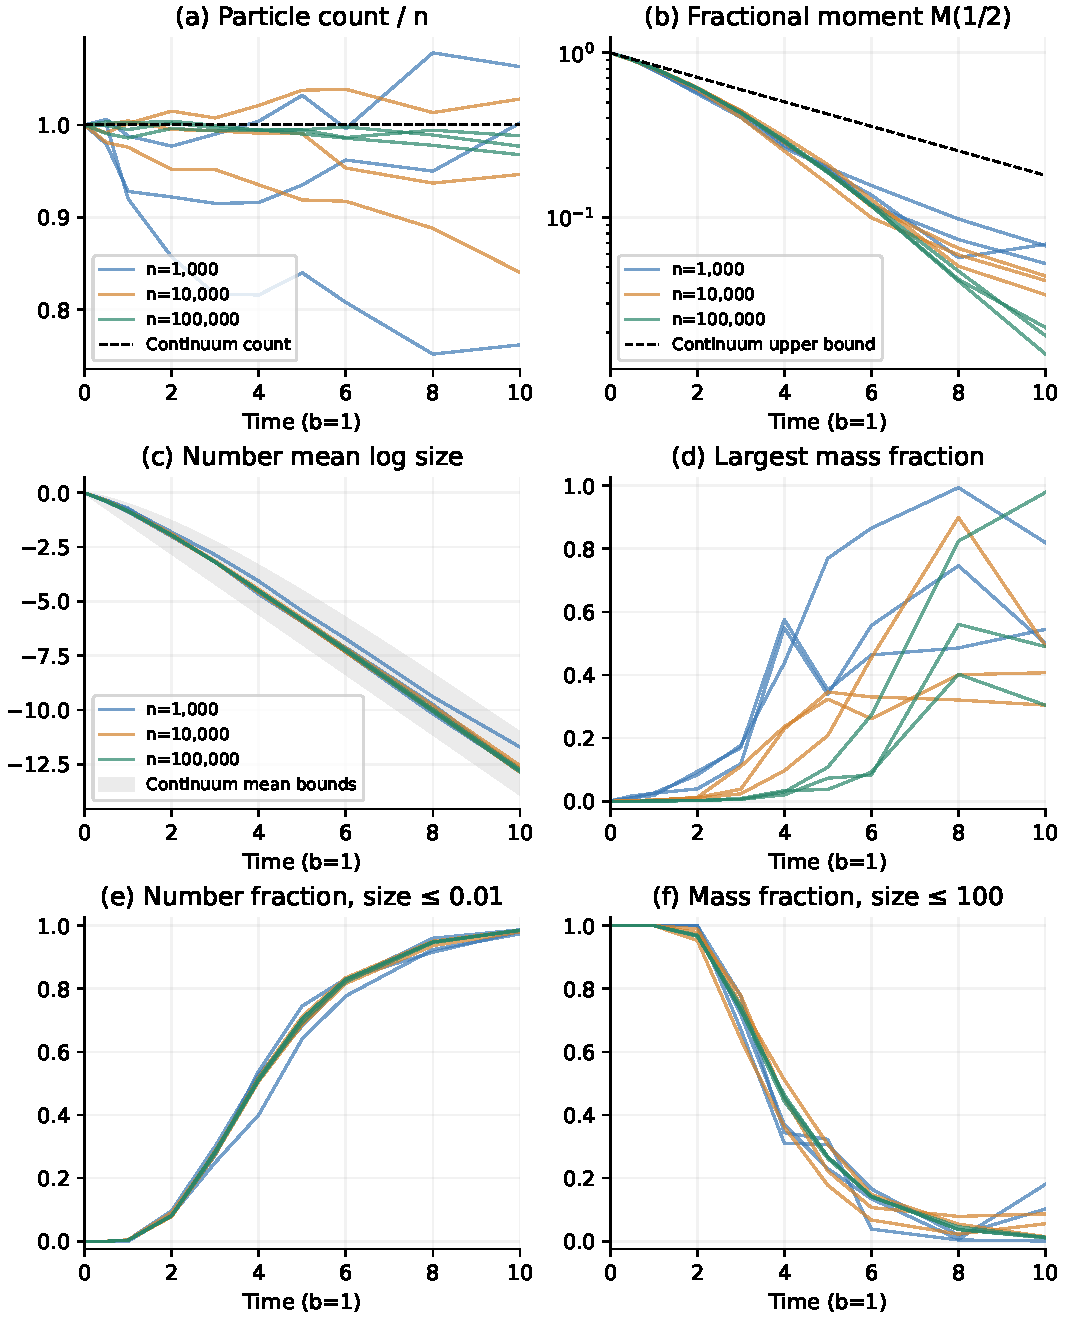
\includegraphics[width=\textwidth,height=.86\textheight,keepaspectratio]{supplement/critical_additive_particles.pdf}
 \caption{All nine finite-particle runs, with three seeds in each color.
 The dashed count and half-moment curves and the shaded mean-log interval
 are continuum references, not pathwise finite-system bounds. Number
 fractions and log means use the actual count $L$; mass fractions use total
 physical mass $n$; $M_{1/2}=n^{-1}\sum_i\sqrt{x_i}$. The figure is generated
 directly from the supplied 90-row CSV.}
 \label{fig:finite-particles}
\end{figure}

\begin{table}[tbp]
 \centering\small
 \begin{tabular}{@{}rrrrr@{}}
 \toprule
 Initial $n$ & $L(10)/n$ & $M_{1/2}(10)$ & Largest mass fraction
 & Number fraction $x\leq0.01$\\
 \midrule
 $10^3$ & $0.762$--$1.063$ & $0.0525$--$0.0688$ & $0.500$--$0.820$ & $0.974$--$0.987$\\
 $10^4$ & $0.8405$--$1.028$ & $0.0339$--$0.0441$ & $0.304$--$0.492$ & $0.981$--$0.986$\\
 $10^5$ & $0.96772$--$0.98823$ & $0.0148$--$0.0215$ & $0.304$--$0.979$ & $0.985$--$0.986$\\
 \bottomrule
 \end{tabular}
 \caption{Minima and maxima over the three declared seeds at time 10.
 These ranges are descriptive, not confidence intervals.}
 \label{tab:finite-particles}
\end{table}

\Cref{fig:finite-particles,tab:finite-particles} show number concentration
near small sizes alongside highly variable material concentration in a few
large particles. At time 10 the count is within $3.3\%$ of its continuum
value for $n=10^5$. The largest absolute relative deviations for $n=10^3$
and $n=10^4$ are $23.8\%$ and $15.95\%$, respectively. The run with
$n=10^4$, seed 47, ends $3.59$ exact standard deviations
below its count mean and is included without selection. Three seeds do not
reliably estimate the count distribution or mass-tail variability. The
dashed half-moment reference is the continuum bound $e^{-\kappa t}$, equal
to $0.17983$ at time 10; the shaded mean-log interval is
$[-2t\log2,\,-2t\log2+(1-e^{-2\kappa t})/(2\kappa)]$ from
\cref{thm:transport} and the half-moment estimate. All nine finite log means
fall inside this interval, but that fact does not turn the interval into a
stochastic bound. The mass-discrepancy certificate of
\cref{thm:finite-discrepancy} at this horizon is about $1.95\times10^{-5}$
for $n=10^3$ and zero for the two larger sizes, whose threshold times
$\log n/\log2$ are $9.97$, $13.29$, and $16.61$ (\cref{rem:finite-constant}).
These runs therefore neither establish a nearly maximal continuum
discrepancy nor measure a first breakdown time.

The half-moment panel does give a rough empirical decay rate. For the
finite system write $A_{1/2}(t)=M_{1/2}(\mu_t^n)$. The fitted rate
$-\log(A_{1/2}(10)/A_{1/2}(4))/6$ on $t\in[4,10]$, computed from the saved
CSV, is listed in \cref{tab:finite-decay}. It is $0.23$--$0.28$ for
$n=10^3$, $0.30$--$0.37$ for $n=10^4$, and $0.43$--$0.50$ for $n=10^5$,
increasing with $n$, against the certified continuum coefficient
$\kappa=3-2\sqrt2\approx0.172$. This supports the conjecture in
\cref{rem:exponent-conjecture} that the true critical exponent for these
data is near $b/2$. The caveats are finite-size effects, including the
ceiling and the $1/n$ correction \eqref{eq:finite-diagonal}, and only three
seeds per size.

\begin{table}[tbp]
 \centering\small
 \begin{tabular}{@{}rrrr@{}}
 \toprule
 Initial $n$ & Seed 11 & Seed 29 & Seed 47\\
 \midrule
 $10^3$ & $0.228$ & $0.275$ & $0.236$\\
 $10^4$ & $0.311$ & $0.368$ & $0.302$\\
 $10^5$ & $0.496$ & $0.432$ & $0.455$\\
 \bottomrule
 \end{tabular}
 \caption{Fitted decay rate $-\log(A_{1/2}(10)/A_{1/2}(4))/6$ of the finite
 half moment on $t\in[4,10]$ with $b=1$, from the saved CSV. The certified
 continuum coefficient is $\kappa\approx0.172$.}
 \label{tab:finite-decay}
\end{table}

The self-contained supplement includes the C++ source, standard-library
Python runner, recorded data and compiler metadata, figure script, and
build commands. Built-in checks exercise selection intervals, resizing,
removal, pair rates, count-generator identities, and conservation over
10,000 events. Each snapshot checks $L=n+\mathrm{births}-\mathrm{deaths}$,
the mass ceiling, and agreement of direct and tree mass sums, with relative
mass tolerance $10^{-10}$. The archived normalized mass is printed as one
at every snapshot. Equal splitting preserves dyadic masses in real
arithmetic, but a bound on their size range does not bound the number of
significant bits needed for exact arithmetic. Floating-point rounding can
occur in merges and cumulative sums even in these runs; the printed mass
values do not certify exact conservation. Longer runs with extreme size
ratios can lose small weights in cumulative sums, and the uniform draws
have 53 bits of resolution. Different
floating-point platforms or C++ library implementations can change a path
with the same seed. The supplement also records the prior independent
structural and count-law checks and their reproducible commands; they are
implementation diagnostics, not extra research trajectories.
